% Template created by Karol Kozioł (www.karol-koziol.net) for ShareLaTeX

\documentclass[a4paper,spanish,9pt]{extarticle}
%%%%
\usepackage[T1]{fontenc}
%%%%
\usepackage[utf8]{inputenc}
\usepackage[spanish]{babel}
\usepackage{lmodern}


%\usepackage[T1]{fontenc}
\usepackage{array}
\usepackage{verbatim}
\usepackage{graphicx}
\usepackage{xcolor}
\newcommand{\degre}{\ensuremath{^\circ}}
\usepackage{pgf,tikz,pgfplots}
\usepackage{import}
\pgfplotsset{compat=1.15}
\usetikzlibrary{shapes, calc, shapes, arrows, math, babel, positioning}

\usepackage{amsmath,amssymb,textcomp,mathrsfs,mathtools}
\everymath{\displaystyle}

\usepackage{times}
\renewcommand\familydefault{\sfdefault}
\usepackage{tgheros}
\usepackage[defaultmono,scale=0.85]{droidmono}

\usepackage{multicol}
\setlength{\columnseprule}{0pt}
\setlength{\columnsep}{20.0pt}

\usepackage[spanish]{babel}
\usepackage{eurosym}


\graphicspath{{./img/}}
%\usepackage{svg}

\usepackage{hyperref}

\usepackage{geometry}
\geometry{
a4paper,
total={210mm,297mm},
left=10mm,right=10mm,top=10mm,bottom=15mm}

\linespread{1.3}

\newcommand{\samedir}{\mathbin{\!/\mkern-5mu/\!}}

% custom title
\makeatletter
\renewcommand*{\maketitle}{%
\noindent
\begin{minipage}{0.6\textwidth}
\begin{tikzpicture}
\node[rectangle,rounded corners=6pt,inner sep=10pt,fill=blue!50!black,text width= 0.95\textwidth] {\color{white}\Huge \@title};
\end{tikzpicture}
\end{minipage}
\hfill
\begin{minipage}{0.35\textwidth}
\begin{tikzpicture}
\node[rectangle,rounded corners=3pt,inner sep=10pt,draw=blue!50!black,text width= 0.95\textwidth] {\begin{tabular}{cc} \multirow{2}{1cm}{
\includegraphics[width=0.15\columnwidth]{header_right}}& \@author \\ & \ies \end{tabular}};
\end{tikzpicture}
\end{minipage}
\bigskip\bigskip
}%
\makeatother

% custom section
\usepackage[explicit]{titlesec}
\newcommand*\sectionlabel{}
\titleformat{\section}
  {\gdef\sectionlabel{}
   \normalfont\sffamily\Large\bfseries\scshape}
  {\gdef\sectionlabel{\thesection\ }}{0pt}
  {
\noindent
\begin{tikzpicture}
\node[rectangle,rounded corners=3pt,inner sep=4pt,fill=blue!50!black,text width= 0.95\columnwidth] {\color{white}\sectionlabel#1};
\end{tikzpicture}
  }
\titlespacing*{\section}{0pt}{15pt}{10pt}


% custom footer
\usepackage{fancyhdr}
\makeatletter
\pagestyle{fancy}
\fancyhead{}
\fancyfoot[C]{\footnotesize \@author \ - \ies}
\renewcommand{\headrulewidth}{0pt}
\renewcommand{\footrulewidth}{0pt}
\makeatother
\usepackage{multirow} % para las tablas


\title{Algebra matricial}
\author{Departamento de Matemáticas}
\date{2014}
\newcommand{\ies}{IES Pedro Cerrada}


\begin{document}

\maketitle



\begin{multicols*}{2}
% Template created by Karol Kozioł (www.karol-koziol.net) for ShareLaTeX

%\documentclass[a4paper,spanish,9pt]{extarticle}
%\usepackage[utf8]{inputenc}
%
%\usepackage[T1]{fontenc}
%\usepackage{verbatim}
%\usepackage{graphicx}
%\usepackage{xcolor}
%\usepackage{pgf,tikz}
%\usepackage{mathrsfs}
%
%\usetikzlibrary{shapes, calc, shapes, arrows, math, babel}
%
%\usepackage{amsmath,amssymb,textcomp}
%\everymath{\displaystyle}
%
%\usepackage{times}
%\renewcommand\familydefault{\sfdefault}
%\usepackage{tgheros}
%\usepackage[defaultmono,scale=0.85]{droidmono}
%
%\usepackage{multicol}
%\setlength{\columnseprule}{0pt}
%\setlength{\columnsep}{20.0pt}
%
%\usepackage[utf8]{inputenc}
%\usepackage[spanish]{babel}
%\usepackage{eurosym}
%
%\usepackage{graphicx}
%\graphicspath{{../img/}}
%\usepackage{svg}
%
%\usepackage{hyperref}
%
%\usepackage{geometry}
%\geometry{
%a4paper,
%total={210mm,297mm},
%left=10mm,right=10mm,top=10mm,bottom=15mm}
%
%\linespread{1.3}
%
%\newcommand{\samedir}{\mathbin{\!/\mkern-5mu/\!}}
%
%% custom title
%\makeatletter
%\renewcommand*{\maketitle}{%
%\noindent
%\begin{minipage}{0.6\textwidth}
%\begin{tikzpicture}
%\node[rectangle,rounded corners=6pt,inner sep=10pt,fill=blue!50!black,text width= 0.95\textwidth] {\color{white}\Huge \@title};
%\end{tikzpicture}
%\end{minipage}
%\hfill
%\begin{minipage}{0.35\textwidth}
%\begin{tikzpicture}
%\node[rectangle,rounded corners=3pt,inner sep=10pt,draw=blue!50!black,text width= 0.95\textwidth] {\begin{tabular}{cc} \multirow{2}{1cm}{
\includegraphics[width=0.15\columnwidth]{header_right}}& \@author \\ & \ies \end{tabular}};
%\end{tikzpicture}
%\end{minipage}
%\bigskip\bigskip
%}%
%\makeatother
%
%% custom section
%\usepackage[explicit]{titlesec}
%\newcommand*\sectionlabel{}
%\titleformat{\section}
%  {\gdef\sectionlabel{}
%   \normalfont\sffamily\Large\bfseries\scshape}
%  {\gdef\sectionlabel{\thesection\ }}{0pt}
%  {
%\noindent
%\begin{tikzpicture}
%\node[rectangle,rounded corners=3pt,inner sep=4pt,fill=blue!50!black,text width= 0.95\columnwidth] {\color{white}\sectionlabel#1};
%\end{tikzpicture}
%  }
%\titlespacing*{\section}{0pt}{15pt}{10pt}
%
%
%% custom footer
%\usepackage{fancyhdr}
%\makeatletter
%\pagestyle{fancy}
%\fancyhead{}
%\fancyfoot[C]{\footnotesize \@author \ - \ies}
%\renewcommand{\headrulewidth}{0pt}
%\renewcommand{\footrulewidth}{0pt}
%\makeatother
%\usepackage{multirow} % para las tablas
%
%
%\title{Funciones}
%\author{Departamento de Matemáticas}
%\date{2014}
%\newcommand{\ies}{IES Pedro Cerrada}
%
%
%
%\begin{document}
%
%\maketitle
%
%
%
%\begin{multicols*}{2}

\section{Conjuntos de números reales}
\subsection{Repaso de Intervalos, Entornos y Valor Absoluto}

\begin{itemize}
\item Se define el \textbf{valor absoluto} de un número como la distancia al cero. Se calcula tomando el número con signo positivo.

\paragraph*{Ejemplos:} 

\begin{tikzpicture}[scale=0.75]
\tikzmath{
			\a = -2; \b = 4; \aa = -3; \bb = 5 ;
			\aabs = -\a; \babs = \b;
          }

\draw[very thick] (\a,0) -- (\b,0);
\path [draw=black, fill=white] (4,0) circle (2pt);
\path [draw=black, fill=white, thick] (-2,0.0) circle (2pt);
\draw[latex-latex] (\a - 1.5,0) -- (\b + 1.5,0) ;

\foreach \x in  {\aa,...,\bb}
\draw[shift={(\x,0)},color=black] (0pt,3pt) -- (0pt,-3pt);
\foreach \x in  {\aa,...,\bb}
\draw[shift={(\x,0)},color=black] (0pt,0pt) -- (0pt,-3pt) node[below] 
{$\pgfmathprintnumber{\x}$};
  \draw[decorate,decoration={brace}, thick]
    (\a,0.2)--(0,0.2) node[above, midway] 
{$\pgfmathprintnumber{\aabs} = |\pgfmathprintnumber{\a}|$}; 
\end{tikzpicture}

\paragraph*{Distancia entre dos números:} Entre $a$ y $b$ hay una distancia de $|a -b|$ 
\paragraph*{Ejemplo:} Determina la distancia entre los números $-2$ y  $4$:

\begin{tikzpicture}[scale=0.75]

\tikzmath{
			\a = -2; \b = 4; \aa = -3; \bb = 5 ;
			\dist = \b - \a;
          }

\draw[very thick] (\a,0) -- (\b,0);
\path [draw=black, fill=white] (4,0) circle (2pt);
\path [draw=black, fill=white, thick] (-2,0.0) circle (2pt);
\draw[latex-latex] (\a - 1.5,0) -- (\b + 1.5,0) ;

\foreach \x in  {\aa,...,\bb}
\draw[shift={(\x,0)},color=black] (0pt,3pt) -- (0pt,-3pt);
\foreach \x in  {\aa,...,\bb}
\draw[shift={(\x,0)},color=black] (0pt,0pt) -- (0pt,-3pt) node[below] 
{$\pgfmathprintnumber{\x}$};
  \draw[decorate,decoration={brace}, thick]
    (-2,0.2)--(4,0.2) node[above, midway] 
{$\pgfmathprintnumber{\dist} = |(\pgfmathprintnumber{\b}) - (\pgfmathprintnumber{\a})|$}; 
\end{tikzpicture}
\end{itemize}



\section{Funciones}

\subsection{Definición}

En el lenguaje matemático se dice que $y$ es \textbf{función} de $x$ cuando $y$ depende de $x$.

\section{Características de una función}

\subsection{Dominio y recorrido}
El conjunto de los posibles valores de la
variable independiente se llama \textbf{dominio de la función} ($Dom(f)$); y el conjunto de valores que toma la variable dependiente, \textbf{imagen o recorrido de la función} ($Im(f)$).

\paragraph{Ejemplo}
$y=x^2$ o $f(x)=x^2$, $x$ es la variable independiente e $y$ es la variable dependiente. El $Dom(f)=\left\lbrace x \in \mathrm{R} | \exists y=f(x)\right\rbrace$ 	

\begin{tikzpicture}[domain=-3:3,>=triangle 45, scale=0.75]

\tikzmath{
			\a = 1/4; \b = 1; \c = -2; 
			\d = 3;
          }
          
\draw[color=red]    plot (\x,{\a*(\x)^2 + \b*\x + \c})             node[right] {$f(x) =\a x^2$}; 
\draw[very thin,color=gray] (-3.5,\c - 0.5) grid (3.5,\a * 3^2 + \b * 3 + \c - 0.1);
\draw[<->] (-3.5,0) -- (3.9,0) node[right] {$x$};
\draw[<->] (0,\c - 0.5) -- (0,\a * 3^2 + \b * 3 + \c) node[above] {$y$};

\end{tikzpicture}

\subsection{Crecimiento y decrecimiento}
\subsection{Cortes con ejes}
\subsection{Funciones acotadas}
\subsection{Funciones periódicas}
\subsection{Funciones inyectivas y biyectivas}
\subsection{Continuidad}
De manera informal, una función es continua si se puede dibujar con un solo trazo, o lo que es lo mismo, sin levantar "del papel" el "bolígrafo". Para dar una definición


\section{Continuidad y límites}
\subsection{Límites en un punto}
Dado $x_0\neq\pm\infty$, decimos que $\lim_{x \to x_0} f(x) = l $ cuando ocurre que si $x$ toma valores próximos al número $x_0$ (tanto menores como mayores), los correspondientes valores de $f (x)$ se aproximan al número $l$

\subsection{Límites laterales}

\subsubsection{Límites por la derecha} Dado $x_0\neq\pm\infty$, decimos que $\lim_{x \to x_0^+} f(x) = l $ cuando ocurre que si $x$ toma valores próximos al número $x_0$ pero  mayores que él, los correspondientes valores de $f (x)$ se aproximan al número $l$

\subsubsection{Límites por la izquierda} Dado $x_0\neq\pm\infty$, decimos que $\lim_{x \to x_0^-} f(x) = l $ cuando ocurre que si $x$ toma valores próximos al número $x_0$ pero  menores que él, los correspondientes valores de $f (x)$ se aproximan al número $l$

\paragraph{Teorema de unicidad del límite:}
Dado $x_0\neq\pm\infty$,
$$\lim_{x \to x_0} f(x) = l \leftrightarrow \lim_{x \to x_0^-} f(x) = \lim_{x \to x_0^+} f(x)= l $$
Por lo tanto si los límites laterales no coinciden, el límite no existe.

\paragraph{Ejemplo:} Calcula el límite de la función $f(x)=\frac{1}{x}$ cuando $x \to 0$.\\
$$\lim_{x \to 0^-} \frac{1}{x} = -\infty$$



    \begin{tabular}{l l}
      Derivatives and Integrals \\
      \\

      Basic Differentiation Rules \\

      \\
      1. $\frac {d}{dx} [cu] = cu'$ & 2. $\frac{d}{dx} [u \pm v] = u' \pm 
      v'$ \\
      3. $\frac{d}{dx} [uv] = uv' + vu'$ & 4. $\frac{d}{dx} [\frac{u}{v}] 
      = \frac{vu' - uv'}{v^2}$ \\
      5. $\frac{d}{dx} [c] = 0$ & 6. $\frac{d}{dx} [u^n] = nu^{n-1} \quad 
      u'$ \\
      7. $\frac{d}{dx} [x] = 1$ & 8. $\frac{d}{dx} [\mid u \mid] = 
      \frac{u}{\mid u \mid} (u'), \quad u \neq 0$ \\
      9. $\frac{d}{dx} [ln \quad u] = \frac{u'}{u}$ & 10. $\frac{d}{dx} 
      [e^u] = e^u \quad u'$ \\
      11. $\frac{d}{dx} [sin \quad u] = (cos \quad u) u'$ & 12. $\frac{d}
      {dx} [cos \quad u] = -(sin \quad u) u'$ \\
      13. $\frac{d}{dx} [tan \quad u] = (sec^2 \quad u)u'$ & 14. 
      $\frac{d}{dx} [cot \quad u] = -(csc^2 \quad u) u'$ \\
      15. $\frac{d}{dx} [sec \quad u] = (sec \quad u \quad tan \quad u) 
      u'$ & 16. $\frac{d}{dx} [csc \quad u] = -(csc \quad u \quad cot 
      \quad u) u'$ \\
      17. $\frac{d}{dx} [arcsin \quad u] = \frac{u'}{\sqrt{-1 - u^2}}$ & 
      18. $\frac{d}{dx} [arccos \quad u] = \frac{-u'}{\sqrt{1-u^2}}$ \\
      19. $\frac{d}{dx} [arctan \quad u] = \frac{u'}{1 + u^2}$ & 20. 
      $\frac{d}{dx} [arccot \quad u] = \frac{-u'}{1 + u^2}$ \\
      21. $\frac{d}{dx} [arcsec \quad u] = \frac{u'}{\mid u \mid 
      \sqrt{u^2 - 1}}$ & 22. $\frac{d}{dx} [arcsec \quad u] = \frac{-u'}
      {\mid u \mid \sqrt{u^2 - 1}}$ \\
      \\
      Basic Integration Formulas \\
      \\
      1. $\int k \quad f(u) \quad d u = k \int f(u) \quad du$ & 2. $\int 
      \quad [f(u) \pm g (u)] \quad du = \int f(u) \quad du \pm \int g(u) 
      \quad du$ \\
      3. $\int  d u = u + C$ & 4. $\int u^n d u = \frac{u^{n+1}}{n + 1} + 
      C, \quad n \neq -1$ \\
      5. $\int \frac{d}{u} = ln \mid u \mid + C$ & 6. $\int e^u d u = e^u 
      + C$ \\
      7. $\int sin \quad u \quad du = -cos u + C$ & 8. $\int cos \quad u 
      \quad d u = sin \quad u + C$ \\
      9. $\int tan \quad u \quad du = -ln \mid cos \quad u \mid + C$ & 
      10. $\int cot \quad u \quad du = ln \mid sin \quad u \mid + C$ \\
      11. $\int sec \quad u \quad du = ln \mid sec \quad u + tan \quad du 
      \mid + C$ & 12. $\int csc \quad u \quad du = -ln \mid csc \quad u + 
      cot \quad u \mid + C$ \\
      13. $\int sec^2 u \quad du  = tan \quad u + C$ & 14. $\int csc^2 
      \quad u \quad du = -cot \quad u + C$ \\
      15. $\int sec \quad u \quad tan \quad u \quad du = sec \quad u + C$ 
      & 16. $\int csc \quad u \quad cot \quad du = -csc \quad u + C$ \\
      17. $\int \frac{du}{\sqrt{a^2 - u^2}} = arcsin \frac{u}{a} + C$ & 
      18. $\int \frac{du}{a^2 + u^2} = \frac{1}{a} arctan \frac{u}{a} + 
      C$ \\
      19. $\int \frac{du}{u \sqrt{u^2 - a^2}} = \frac{1}{a} arcsec 
      \frac{\mid u \mid}{a} + C$ \\

  \end{tabular}


\usetikzlibrary{arrows,intersections}
\tikzpicture[scale=0.5,
        thick,
        >=stealth',
        dot/.style = {
            draw,
            fill=white,
            circle,
            inner sep=0pt,
            minimum size=4pt
        }
    ]
    \coordinate (O) at (0,0);
    \draw[->] (-0.3,0) -- (8,0) coordinate[label={below:$x$}] (xmax);
    \draw[->] (0,-0.3) -- (0,5) coordinate[label={right:$f(x)$}] (ymax);
    \path[name path=x] (0.3,0.5) -- (6.7,4.7);
    \path[name path=y] plot[smooth] coordinates {(-0.3,2) (2,1.5) (4,2.8) (6,5)};
    \scope[name intersections={of=x and y,name=i}]
        \fill[gray!20] (i-1) -- (i-2 |- i-1) -- (i-2) -- cycle;
        \draw (0.3,0.5) -- (6.7,4.7) node[pos=0.8,below right] {Sekante};
        \draw[red] plot[smooth] coordinates {(-0.3,2) (2,1.5) (4,2.8) (6,5)};
        \draw (i-1) node[dot,label={above:$P$}] (i-1) {} -- node[left] {$f(x_0)$} (i-1 |- O) node[dot,label={below:$x_0$}] {};
        \path (i-2) node[dot,label={above:$Q$}] (i-2) {} -- (i-2 |- i-1) node[dot] (i-12) {};
        \draw (i-12) -- (i-12 |- O) node[dot,label={below:$x_0 + \varepsilon$}] {};
        \draw[blue,<->] (i-2) -- node[right] {$f(x_0 + \varepsilon) - f(x_0)$} (i-12);
        \draw[blue,<->] (i-1) -- node[below] {$\varepsilon$} (i-12);
        \path (i-1 |- O) -- node[below] {$\varepsilon$} (i-2 |- O);
        \draw[gray] (i-2) -- (i-2 -| xmax);
        \draw[gray,<->] ([xshift=-0.5cm]i-2 -| xmax) -- node[fill=white] {$f(x_0 + \varepsilon)$}  ([xshift=-0.5cm]xmax);
    \endscope
\endtikzpicture

\newpage


\begin{tabular}{|c|c|}\hline 
Función  & Derivada  \\ 
\hline
$f(x) = k$  & $f'(x) = 0$   \\ 
$f(x) = x$  &                     $f'(x)= 1$ \\
$f(x) = x^n$ &                    $f'(x)= n\cdot x^{n-1}$\\
$f(x) = \sqrt x $ &      $f'(x)$= $\frac{1}{{2\sqrt x }}$\\
$f(x) = \sqrt[n]{x}$  &     $f'(x)$= $\frac{1}{n\cdot\sqrt[n]{x^{n - 1}}}$\\
$f(x) = \ln{x}$ &                  $f'(x)= \frac{1}{x}$\\
$f(x) = \log_a x$ &              $f'(x)=\frac{1}{x}\cdot\frac{1}{\ln a}$\\
$f(x) = e^x$ &                     $f'(x)=e^x$\\
$f(x) = a^x$ &                     $f'(x)= a^x\cdot\ln a$\\
$f(x) = \sin x$ &               $f'(x)= \cos x$ \\
$f(x) = \cos x$  &              $f'(x)= -\sin x$\\
$f(x) = \tan x$ &                  $f'(x)$= $\frac{1}{{{{\cos }^2}x}}$\\
%f(x) = cotg x              $f'(x)$= $\frac{{ - 1}}{{se{n^2}x}}{\text{ }} = {\text{  -  cose}}{{\text{c}}^{\text{2}}}x$
%f(x) = sec x                $f'(x)$= tg x . sec x
%f(x) = cosec x            $f'(x)$= -cotg x . cosec x
%f(x) = arc sen x        $f'(x)$= $\frac{1}{{\sqrt {1 - {x^2}} }}$
%f(x) = arc cos x         $f'(x)$= $\frac{{ - 1}}{{\sqrt {1 - {x^2}} }}$
%f(x) = arc tg x           $f'(x)$= $\frac{1}{{1 + {x^2}}}$
%f(x) = arc cotg x       $f'(x)$= $\frac{{ - 1}}{{1 + {x^2}}}$
\hline

\end{tabular} 

\begin{tabular}{|c|}\hline 
Operaciones con derivadas  \\ 
\hline
$y=u + v \rightarrow y' = u' + v'$    \\ 
$y=u - v \rightarrow y' = u' - v'$    \\
$y=K\cdot u \rightarrow y' = K \cdot u'$    \\ 
$y=u \cdot v \rightarrow y' = u'\cdot v + u\cdot v'$    \\
$y= \frac{u}{v}  \rightarrow y' = \frac{u'\cdot v - u\cdot v'}{v^2}$    \\  
\hline

\end{tabular} 

\paragraph{Regla de la cadena} Dada una función compuesta: 

$$\left(g \circ f\right)'(x)=g'\left(f(x)\right)\cdot f'\left(x\right) $$  

\subparagraph{Ejemplo}

Dado la función $f(x)$

     




%\end{multicols*}
%
%\end{document}

%\section{Variables aleatorias y distribuciones de probabilidad}

\paragraph{Finalidad :} Abstraer matemáticamente un tipo de experimento aleatorio. Y, con ello, poder estimar de manera teórica lo que sucedería de manera experimental mediante una estadística. 

\paragraph{¿Cómo?:} Mediante variables aleatorias y distribuciones de probabilidad asociadas a esas variables:

\section{Variables aleatorias} Una variable aleatoria es una función que a cada suceso
elemental de un espacio muestral le asigna un número. Para hacer referencia a las variables se usan las letras: $X$, $Y$, ...

\paragraph{Ejemplo:} Sea el experimento aleatorio “lanzar un dado”: El espacio muestral lo componen las 6 caras del dado. Podemos asignar la variable $X$ que a cada cara le asocia el número que represente su cara.

\begin{center}
\begin{tabular}{ccc}
 & $X$ &  \\
Suceso &  &  $x_i$\\ \hline 
Cara 1 & $\rightarrow$ & 1 \\ 
Cara 2 & $\rightarrow$ & 2 \\ 
Cara 3 & $\rightarrow$ & 3 \\ 
Cara 4 & $\rightarrow$ & 4 \\ 
Cara 5 & $\rightarrow$ & 5 \\ 
Cara 6 & $\rightarrow$ & 6 \\ 
\end{tabular} 
\end{center}

\paragraph{Ejemplo:} Sea el experimento compuesto lanzar dos monedas. Podemos asignar la variable aleatoria: $$Y=\left\lbrace Número \ de \ caras \right\rbrace$$

\begin{center}
\begin{tabular}{ccc}
 & $Y$ &  \\
Suceso &  &  $y_i$\\ \hline 
C,C & $\rightarrow$ & 2 \\ 
C,X & $\rightarrow$ & 1 \\ 
X,C & $\rightarrow$ & 1 \\ 
X,X & $\rightarrow$ & 0 \\ 
\end{tabular} 
\end{center}

\subsection{Tipos de variables aleatorias}
\begin{description}
\item[Discretas:] Toman un número finito o numerable de valores
\item[Continuas:] Toman valores en un rango continuo
\end{description}

\paragraph{Ejemplo de variables discreta:} Sea la \emph{X =“El número de caras al lanzar dos dados”}. Los valores posibles son 0, 1 o 2 (que es un conjunto finito de datos, en concreto 3 datos) 

\paragraph{Ejemplo de variables continua:} \emph{X = “Distancia al centro de la diana medida desde la posición en que cae un dardo lanzado por un tirador experto” }. En este caso la variable puede tomar cualquier valor en el rango entre 0 y el radio de la diana 

\section{Distribuciones de probabilidad}

Llamaremos Distribución de probabilidad a la relación entre los valores de la variable y sus probabilidades.

Estas relaciones se pueden indicar mediante el uso de funciones. El tipo de función y su tratamiento es diferente según las variables sean discretas o continuas.

Veamos algunas distribuciones:


\section{Distribución uniforme discreta}

\paragraph{Ejemplo: } Sea la variable \emph{X = “Número obtenido al lanzar una dado”}\\
A cada valor de la variable podemos asignarle su probabilidad:

%\begin{center}
%\begin{tabular}{ccc}
% & $P(X)$ &  \\
%Suceso &  &  $y_i$ \\ \hline 
%1 & $\rightarrow$ & \frac{1}{6} \\ 
%2 & $\rightarrow$ & \frac{1}{6} \\ 
%3 & $\rightarrow$ & \frac{1}{6} \\ 
%4 & $\rightarrow$ & \frac{1}{6} \\ 
%5 & $\rightarrow$ & \frac{1}{6} \\ 
%6 & $\rightarrow$ & \frac{1}{6} \\ 
%\end{tabular} 
%\end{center}

\begin{center}
\begin{tabular}{ccc}
 & $P(X)$ &  \\
$x_i$ &  &  $P(x_i)$\\ \hline 
1 & $\rightarrow$ & $\tfrac{1}{6}$ \\ 
2 & $\rightarrow$ & $\tfrac{1}{6}$ \\ 
3 & $\rightarrow$ & $\tfrac{1}{6}$ \\ 
4 & $\rightarrow$ & $\tfrac{1}{6}$ \\ 
5 & $\rightarrow$ & $\tfrac{1}{6}$ \\ 
6 & $\rightarrow$ & $\tfrac{1}{6}$ \\ 
\end{tabular} 
\end{center}

Podemos representar la relación anterior mediante una función:

%$$f\colon \begin{array}{lc} 
%         & X \rightarrow Y \\ 
%         & x \mapsto f(x)=\frac{x-1}{2} 
%         \end{array}$$
%
%
%$$f\colon \begin{array}{>{\displaystyle}l} 
%          X \rightarrow Y \\ 
%          x\mapsto f(x)=\frac{x-1}{2} 
%         \end{array}$$

$$P\colon \begin{array}{ll} 
          X \rightarrow \mathbb{R} \\ 
          x_i\mapsto P(X=x_i)=\frac{1}{n} 
         \end{array}$$

Todas las caras tienen la misma probabilidad: $\frac{1}{n}$, siendo $n$ el número de caras, o tamaño del espacio muestral. 

A este tipo de distribución se le llama \textbf{uniforme discreta}.

\section{Distribución Binomial}

\paragraph{Ejemplo:} Queremos calcular las probabilidades de que al lanzar 5 monedas, obtengamos tres caras.
Un suceso que cumple el enunciado es:
$$S_1=\left\lbrace C,C,C,X,X \right\rbrace$$
Teniendo en cuenta que lanzar cada moneda son experimentos independientes, la probabilidad de ese suceso será:
%$$P\left(S_1\right)=P\left(C_1\right)\cdot P\left(C_2 C_1 \right)$$
\begin{eqnarray*}
P\left(S_1\right) & = &P\left(C_1\right)\cdot P\left(C_2 | C_1 \right)\cdot ... \cdot P\left(X_5 | C_1 \cap C_2  \cap C_3  \cap X_4   \right)= \\ &  = & P\left(C_1\right)\cdot  P\left(C_2\right) \cdot P\left(C_3\right) \cdot P\left(X_4\right) \cdot P\left(X_5\right)= \\
& = & P\left(C\right)^3\cdot  P\left(X\right)^2
\end{eqnarray*}

Como la probabilidad de que una moneda sea cara es $\frac{1}{2}$ y la de que sea cruz también:

$$P\left(S_1\right)=\left(\frac{1}{2}\right)^3\cdot  \left(\frac{1}{2}\right)^2$$

Ahora bien, habrá tantos sucesos que cumplan el enunciado como combinaciones de 5 elementos tomados de 3 en 3. Por tanto la probabilidad de que salgan 3 caras será:

$$P\left(Salgan \ 3 \ caras\right)=\binom{5}{3}\left(\frac{1}{2}\right)^3\cdot  \left(\frac{1}{2}\right)^2$$

Si asociamos al experimento "lanzar 5 monedas" le asignamos la variable "número de caras obtenidas", podemos determinar la probabilidad mediante la siguiente función.

$$P\colon \begin{array}{l} 
          X \rightarrow \mathbb{R} \\ 
          k\mapsto P(X=k)=\binom{5}{k}\left(\frac{1}{2}\right)^k\cdot  \left(\frac{1}{2}\right)^{5-k} 
         \end{array}$$

Esto es un ejemplo de distribución binomial de tamaño $5$ y probabilidad $0.5$ .

Realizando los cálculos para $k = 1,...,5 $, la distribución de probabilidad de $X$ que resulta es:

\begin{center}
\begin{tabular}{ccc}
 & $P(X)$ &  \\
$x_i$ &  &  $P(x_i)$\\ \hline 
0 & $\rightarrow$ & $0.03125$ \\ 
1 & $\rightarrow$ & $0.15625$ \\ 
2 & $\rightarrow$ & $0.3125$ \\ 
3 & $\rightarrow$ & $0.3125$ \\ 
4 & $\rightarrow$ & $0.15625$ \\ 
5 & $\rightarrow$ & $0.03125$ \\ 
\end{tabular} 
\end{center}

Y gráficamente: 

%\documentclass{article}
%\usepackage{pgfplots}
%\pgfplotsset{compat=1.7}
%
%\begin{document}
\begin{tikzpicture}[
    declare function={binom(\k,\n,\p)=\n!/(\k!*(\n-\k)!)*\p^\k*(1-\p)^(\n-\k);}
]
\begin{axis}[
    samples at={0,...,5},
    yticklabel style={
        /pgf/number format/fixed,
        /pgf/number format/fixed zerofill,
        /pgf/number format/precision=1
    },
    ybar=0pt, bar width=1
]
\addplot [fill=cyan, fill opacity=0.5] {binom(x,5,0.5)}; \addlegendentry{$p=0.5$}

\end{axis}
\end{tikzpicture}
%\end{document}


\paragraph{Generalización de distribución Binomial:} Hablaremos de una distribución binomial cuando:
\begin{itemize}
\item Se parte de un experimento compuesto de varios simples independientes
\item Los experimentos simples son dicotómicos. Es decir, solo puede haber dos sucesos elementales: uno al que llamaremos acierto y otro al que llamaremos fracaso
\item Asociado al experimento compuesto tenemos la variable número de aciertos cuando realizamos el experimento simple un número determinado de veces
\end{itemize}

En la situación anterior, la distribución binomial vendrá determinada por dos parámetros:
\begin{itemize}
\item Parámetro $n$: Número de veces que se realiza el experimento simple 
\item Parámetro $p$: La probabilidad de que ocurra el suceso acierto
\end{itemize}


A este tipo de variable y su distribución de probabilidades se le llama binomial. \\


\paragraph{Ejemplo:} Así en el ejemplo de las monedas, el experimento se compone de \textbf{5 lanzamientos de moneda}. Si sale cara es acierto y si no fracaso. La variable aleatoria asociada al experimento será el número de caras que salen al lanzar 5 monedas. Esta variable sigue una distribución binomial.

\subsection{Probabilidad de la binomial}\textbf{En general tendremos una binomial de tamaño $n$ y probabilidad $p$}, cuando el experimento simple se haga $n$ veces y la probabilidad de acierto sea $p$.

La función de probabilidad en este caso nos queda:
 
 $$P\colon \begin{array}{l} 
          X \rightarrow \mathbb{R} \\ 
          k\mapsto P(X=k)=\binom{n}{k}\left(p\right)^k\cdot  \left(1-p\right)^{n-k} 
         \end{array}$$
         
\paragraph{Ejemplos:} Representación gráfica de algunas binomiales:    
         
%\documentclass{article}
%\usepackage{pgfplots}
%
%\begin{document}
\begin{tikzpicture}[
    declare function={binom(\k,\n,\p)=\n!/(\k!*(\n-\k)!)*\p^\k*(1-\p)^(\n-\k);}
]
\begin{axis}[
    samples at={0,...,40},
    yticklabel style={
        /pgf/number format/fixed,
        /pgf/number format/fixed zerofill,
        /pgf/number format/precision=1
    }
]
\addplot [only marks, cyan] {binom(x,40,0.2)}; \addlegendentry{$p=0.2 \, n=40$}
\addplot [only marks, orange] {binom(x,40,0.5)}; \addlegendentry{$p=0.5 \, n=40 $}
\end{axis}
\end{tikzpicture}
%\end{document}
         
 

\section{Distribución Normal}
Se trata de una distribución asociada a a un variable continua. Tiene dos parámetros:
\begin{itemize}
    \item $\mu :$ Media de la distribución
    \item $\sigma :$ Desviación típica
\end{itemize}
Y se denota así: $
X \sim \mathcal{N}(\mu,\,\sigma)\,.
    $ 
    
La probabilidad total es 1 y la variable $X$ puede tomar $\infty$ valores ($x \in \left(-\infty, +\infty\right)$). Por tanto, en variables continuas la probabilidad de que tome un valor concreto será 0 ($\lim_{x \to \infty}\frac{1}{x}=0$).    

\subsection{función de densidad de una variable continua:}  En variables continuas solo tiene sentido calcular la probabilidad en intervalos.
Se llama \textbf{función de densidad} ($f(x)$) aquella que: 

$$P\left(a\leq X \leq b \right) = \int_{a}^{b} f(x) dx$$

La interpretación gráfica de lo anterior nos dice que la probabilidad de un intervalo corresponde con el área de la función de densidad en ese intervalo.

%\documentclass{article}
%\usepackage{pgfplots}
%\usetikzlibrary{math}
%\begin{document}



\begin{tikzpicture}[scale=0.7]

\pgfmathdeclarefunction{gauss}{2}{%
  \pgfmathparse{1/(#2*sqrt(2*pi))*exp(-((x-#1)^2)/(2*#2^2))}%
}

\tikzmath{
			\conf = 0.96; \crit= 2.05; \a=round(1-\conf)/2,2);
          }

%\begin{axis}[
%  no markers, domain=0:10, samples=100,
%  axis lines*=left, xlabel=$x$, ylabel=$y$,
%  every axis y label/.style={at=(current axis.above origin),anchor=south},
%  every axis x label/.style={at=(current axis.right of origin),anchor=west},
%  height=5cm, width=12cm,
%  xtick={4,6.5}, ytick=\empty,
%  enlargelimits=false, clip=false, axis on top,
%  grid = major
%  ]
%  \addplot [fill=cyan!20, draw=none, domain=0:5.96] {gauss(6.5,1)} \closedcycle;
%  \addplot [very thick,cyan!50!black] {gauss(4,1)};
%  \addplot [very thick,cyan!50!black] {gauss(6.5,1)};
%
%
%%\draw [yshift=-0.6cm, latex-latex](axis cs:4,0) -- node [fill=white] {$1.96\sigma$} (axis cs:5.96,0);
%\end{axis}

\begin{axis}[
  no markers, domain=-5:5, samples=100,
  axis lines=left, 
  %xlabel=$xa$, ylabel=$ya$,
  %every axis y label/.style={at=(current axis.above origin),anchor=south},
  %every axis x label/.style={at=(current axis.right of origin),anchor=west},
  height=5cm, width=12cm,
  xtick={-1,\crit}, ytick=\empty,
  xticklabels = {$a$, $b$},
  enlargelimits=false, clip=false, axis on top,
  %grid = major
  ]
  \addplot [fill=cyan!20, draw=none, domain=-1:\crit] {gauss(0,1)} \closedcycle;
  \addplot [very thick,cyan!50!black] {gauss(0,1)};
  %\addplot [very thick,cyan!50!black] {gauss(6.5,1)};
  


%\draw [yshift=-0.6cm, latex-latex](axis cs:4,0) -- node [fill=white] {$1.96\sigma$} (axis cs:5.96,0);
\end{axis}
\node[] at (5.5,1.5) {$P\left(a\leq X \leq b \right) $};	




\end{tikzpicture}

%\end{document}

\subsection{función de densidad de una distribución normal:}  En el caso de una $
X \sim \mathcal{N}(\mu,\,\sigma)
    $, la función de densidad es:
    $$f(x)=\frac{1}{{\sigma \sqrt {2\pi } }}e^{{{ - \left( {x - \mu } \right)^2 } \mathord{\left/ {\vphantom {{ - \left( {x - \mu } \right)^2 } {2\sigma ^2 }}} \right. \kern-\nulldelimiterspace} {2\sigma ^2 }}}$$
\paragraph{Ejemplos de representaciones gráficas de normales:} 
%\documentclass{article}
%\usepackage{pgfplots}
%\begin{document}



\begin{tikzpicture}
\pgfmathdeclarefunction{gauss}{2}{%
  \pgfmathparse{1/(#2*sqrt(2*pi))*exp(-((x-#1)^2)/(2*#2^2))}%
}

\begin{axis}[every axis plot post/.append style={
  mark=none,domain=-2:3,samples=50,smooth}, % All plots: from -2:2, 50 samples, smooth, no marks
  axis x line*=bottom, % no box around the plot, only x and y axis
  axis y line*=left, % the * suppresses the arrow tips
  enlargelimits=upper] % extend the axes a bit to the right and top
  \addplot {gauss(0,0.5)};
  \addlegendentry{$\mu=0 \land \sigma^{2}=0.5$}
  \addplot {gauss(1,0.75)};
  \addlegendentry{$\mu=1 \land \sigma^{2}=0.75$}
  \addplot {gauss(0,1)};
  \addlegendentry{$\mu=0 \land \sigma^{2}=1$}
\end{axis}
\end{tikzpicture}


%\end{document}

\subsection{Cálculo práctico de la probabilidad de la Normal:} En realidad, para calcular la probabilidad no se hace la integral, sino que se utiliza una tabla que ya tiene calculadas probabilidades de la  $Z \sim \mathcal{N}(0,\,1)\,.
    $.
%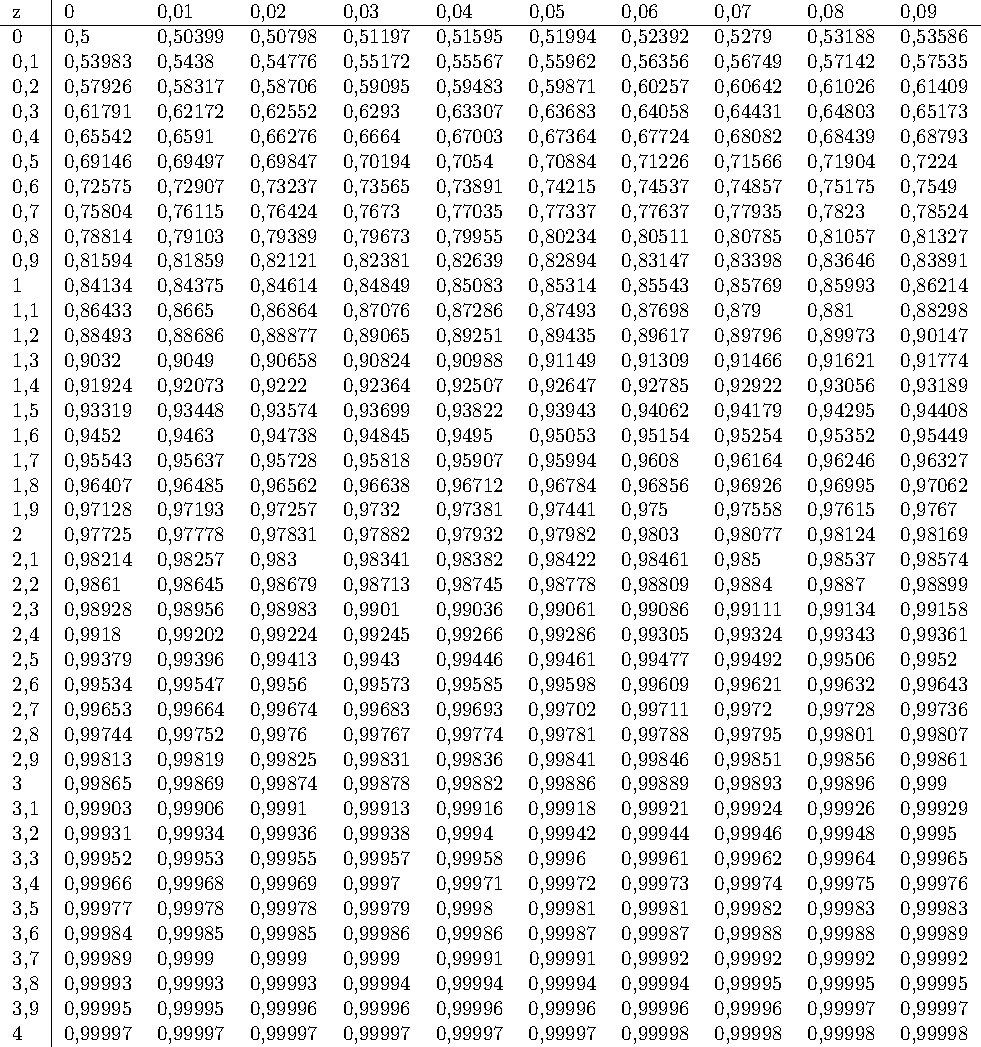
\includepdf[pages=-, scale=0.9]{distribucion_normal.pdf}

%\documentclass{article}
%\usepackage{pgfplots}
%\begin{document}



\begin{tikzpicture}

\pgfmathdeclarefunction{gauss}{2}{%
  \pgfmathparse{1/(#2*sqrt(2*pi))*exp(-((x-#1)^2)/(2*#2^2))}%
}

\begin{axis}[
  no markers, domain=0:10, samples=100,
  axis lines*=left, xlabel=$x$, ylabel=$y$,
  every axis y label/.style={at=(current axis.above origin),anchor=south},
  every axis x label/.style={at=(current axis.right of origin),anchor=west},
  height=5cm, width=12cm,
  xtick={4,6.5}, ytick=\empty,
  enlargelimits=false, clip=false, axis on top,
  grid = major
  ]
  \addplot [fill=cyan!20, draw=none, domain=0:5.96] {gauss(6.5,1)} \closedcycle;
  \addplot [very thick,cyan!50!black] {gauss(4,1)};
  \addplot [very thick,cyan!50!black] {gauss(6.5,1)};


\draw [yshift=-0.6cm, latex-latex](axis cs:4,0) -- node [fill=white] {$1.96\sigma$} (axis cs:5.96,0);
\end{axis}

\end{tikzpicture}

%\end{document}











%\import{probabilidad/}{probabilidad}


\end{multicols*}

\end{document}
